\documentclass[11pt]{article}

%Abstract (10 lines, specific approach and results) -> Henrique
%1. Introduction -> Maurijn
%2. Architecture (all software components + interfaces) -> Henrique
%3. Implementation (how you did it, and who did what)
%	Communication -> Maurijn
%	Log -> Maurijn
%	LPF -> Enrico
%	Kalman -> Enrico
%	Full Control -> Enrico
%	Yaw Control -> Enrico
%	PC side (User interface + User input)-> Enrico
%	Manual mode -> Henrique
%	calibration mode -> Henrique
%	clip function -> Henrique
%	Wireless -> Maurijn
%4. Experimental results -> Maurijn
%5. Conclusion (evaluate design, team results, individual performance, learning experience) -> Henrique
%Appendices (all component interfaces, component code for those components you wish to feature)


\title{\vspace*{-1cm}{\bf IN4073 Technical Report 2011-2012}}
\author{	\textbf{Team G} \\
			E. Caruso (4204395) \\
			H.N. Dantas (4172922) \\
			M. Neumann (1267264)}
\date{April 2012}

\usepackage{vmargin}
\setpapersize{A4}
\setmarginsrb{1.8cm}{1cm}{1.8cm}{2cm}%
{\baselineskip}{\baselineskip}{baselineskip}{\baselineskip}

\usepackage{verbatim}
\usepackage{amsmath}
\usepackage{graphicx}
\usepackage[]{units}
\usepackage[pdftex]{hyperref}
\hypersetup
{
        colorlinks=true,
        linkcolor=black,       % \ref{...} and \pageref{...}
        urlcolor=black,       % \href{...}{...} external (URL)
        filecolor=black,     % \href{...} local file
        pdftitle={IN4073 Technical Report 2011-2012},
        pdfauthor={E. Caruso, H. Dantas, M. Neumann},
        pdfsubject={ERTS},
        pdfkeywords={Quad Rotor,Embedded programming,UAV,Control,C,IN4073 ERTS,EWI,TU Delft},
        pdfproducer={pdfLaTeX},
        bookmarksopen=true,
        pdfborder={0 0 0}
}

\begin{document}

\maketitle

\begin{abstract}
%Abstract (10 lines, specific approach and results)
For the ERTS course was necessary to design, develop and test a control system for a quad rotor (QR). The controller should be able to stabilize the vehicle and respond to the pilot commands.
 
A protocol was invented by the team to address the communication needs of this project. Close attention was paid to the strict bandwidth constraints and exigent reliability requirements.

In order to control the vehicle, it was equipped with an accelerometer, a gyroscope and a FPGA.
Due to high noise on the sensor readings two filters were implemented, Butterworth and Kalman. The former used for yaw control, and the latter for pitch and roll stabilization.

Telemetry data is displayed on the PC in real-time. Additionally, a log file with extensive information is kept during flight and sent to the PC upon request.

During demonstration the controller proved to be very fast and accurate, with latencies in the order of $\mu$-seconds which resulted in a quasi-static behavior of the quad rotor, as desired.
 
\end{abstract}

\section{Introduction}
The IN4073 Embedded Real-Time Systems course presents its students with several unmanned aerial vehicles (UAVs), controlled through four rotors. Fittingly, these devices are called quad rotor aerial vehicles or QRs for short. The appeal of the prospect of being rewarded with 6 credits for piloting such a craft is somewhat lessened due to the ease with which said craft inflicts bodily harm or self-destructs by flying into walls and ceilings. The complete lack of any kind of control requires superhuman pilot abilities to compensate for the QR instability.

This report describes the design, development and testing of a control system for the QR. The overall goal was to enable an inexperienced pilot to fly without the risk for repercussions -- be they medical, financial or educational in nature. As such focus was on reliability and robustness. The process was complicated by limited access to the device, as well as its limited capabilities.

The document is structured as follows. The following section details the software architecture in use. Section~\ref{sec:implementation} documents various components in-depth. Experimental results can be found in Section~\ref{sec:experimental}. Conclusions are drawn in the final section.

\section{Architecture}
\label{sec:architecture}


To control this vehicle it was found necessary to define a high-level architecture that fulfills two main goals: develop various modules that although independent, work together and reduce the computing efforts of the QR as much as possible.

The former provided an organized and easy to understand code; necessary to avoid bugs. Moreover it allowed an even distribution of the workload by the members of the group. Also important: changes in one particular block would not affect the remainder.

The latter is due to the limited computational capabilities of the x32 soft-core running on the FPGA. It is important to note that the UAV should be able to handle communication errors and in case of problems land autonomously. This necessitates that most computations are done on board. However, some of the important computations can be offloaded to the PC.

The diagram representing the approach chosen is depicted in Figure~\ref{fig:block}.

\begin{figure}[ht]
\centering
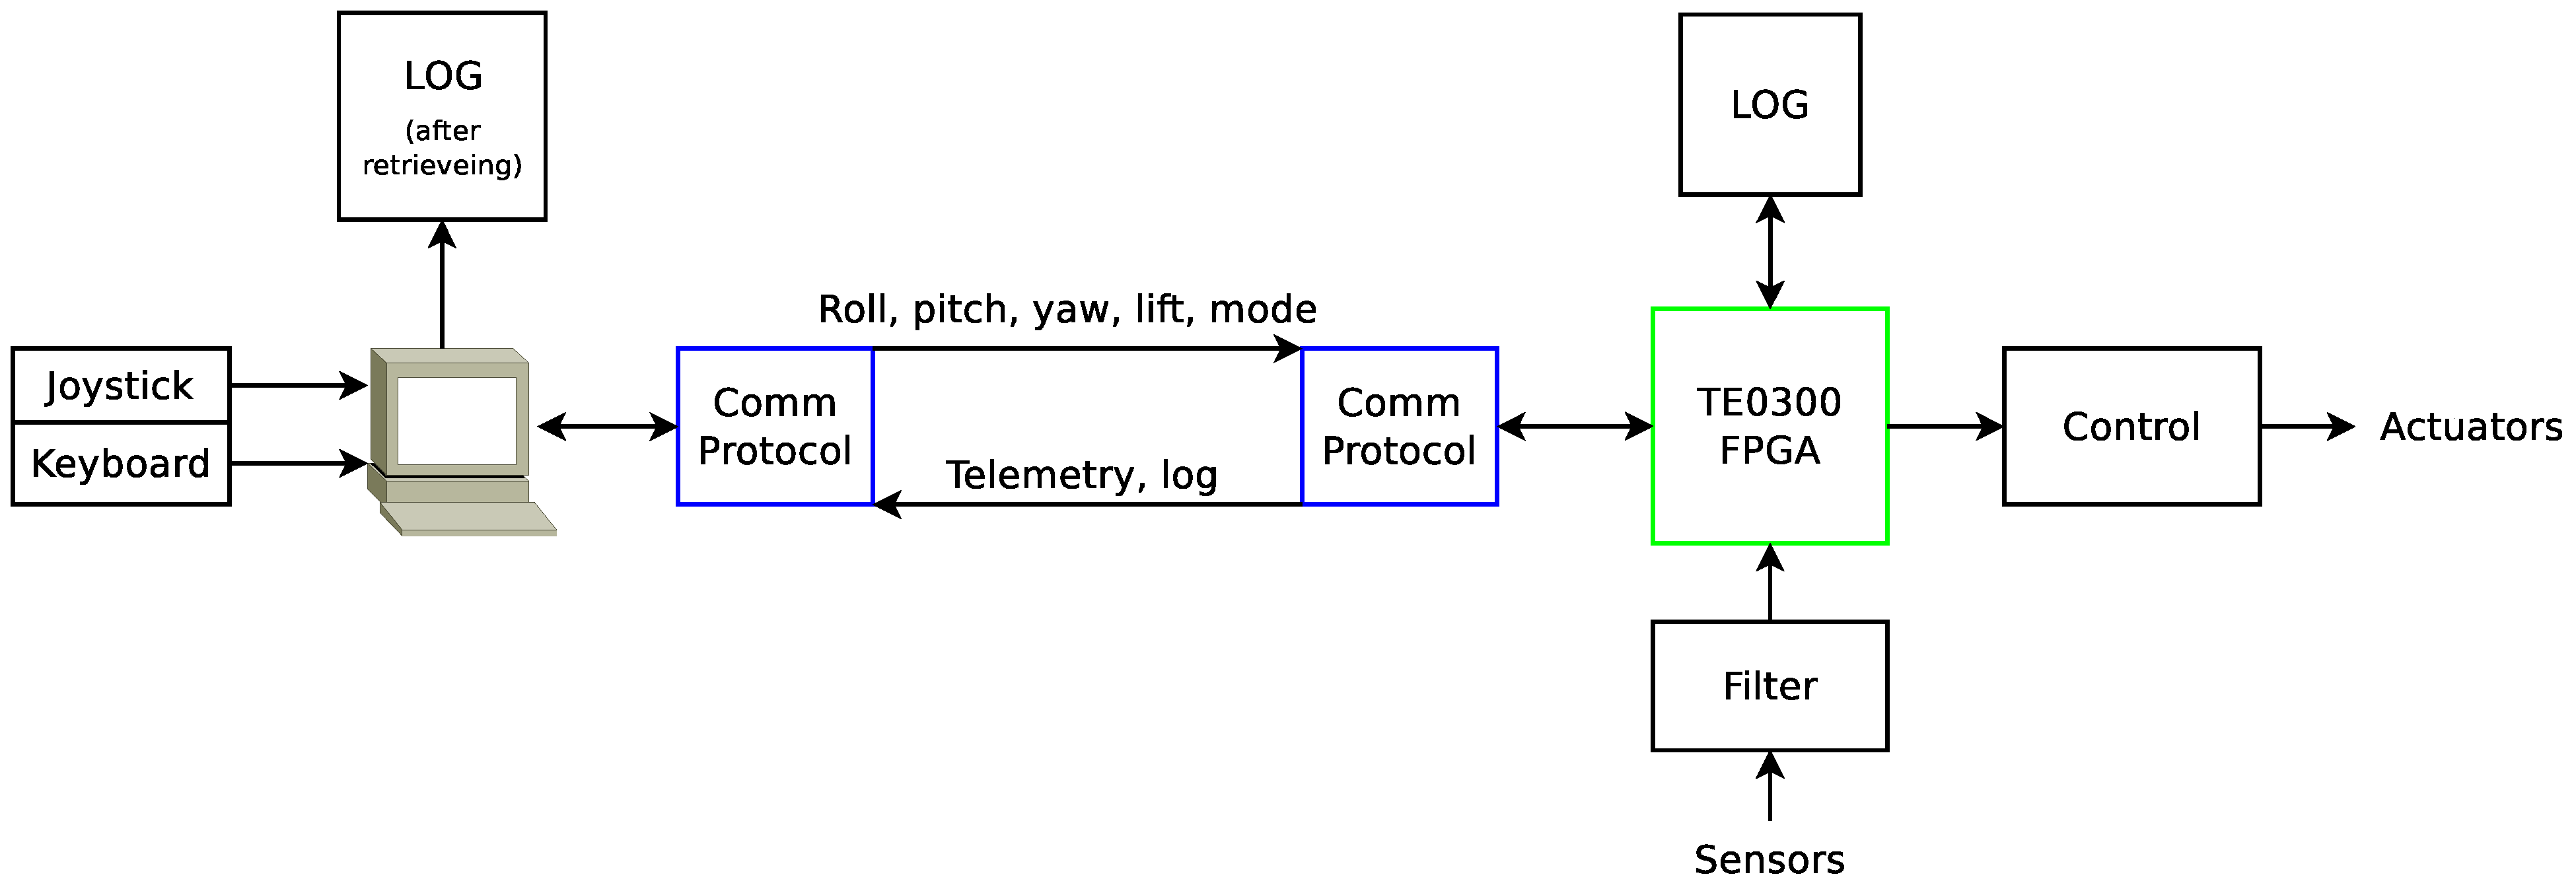
\includegraphics[width=0.9\textwidth,keepaspectratio=true,height=0.3\textheight]{blockdiagram}
\caption{Block diagram of the apparatus' software and hardware components.}
\label{fig:block}
\end{figure}

The commands from the user are sent through the keyboard and the joystick and are handled by the PC when it detects an appropriate event. This information is then communicated to the QR in the form of roll, pitch, yaw and lift, request for mode change or controller tuning.
The communication protocol was developed to ensure maximum reliability and minimum overhead, due to limited bandwidth. This block interfaces with the others through the two functions responsible for sending and receiving data in the PC and the QR.
The computer side is also capable of reading and displaying the telemetry information on the display. This data includes sensor values, engine speed and other relevant information.
The log block on the PC encapsulates the functions used to retrieve and save the log information sent by the quad rotor. On the other hand, the QR log implements routines that save in memory various types of data and handles the request and transmission of that information.
The filters used were Butterworth and Kalman which reduce the noise of ``raw'' accelerometer and gyroscope readings. These filtered signals are consequently used by the control functions represented by the block of the same name.
This determines the desired roll, pitch, yaw and lift given the filtered signals and the user commands which are consequently converted to engine speed.

\section{Implementation}
\label{sec:implementation}
Though work was distributed as intended everyone ended up having many fingers in many pies. As such a work distribution table is difficult to produce. Roughly speaking, M. Neumann was responsible for the communication and log; E. Caruso was responsible for filters and input. Finally, H. Dantas' had a large part in control structure, various modes and the many safety functions.

\subsection{Communication}
For interaction between the PC and QR a communication protocol is required. Reliability is the key design aspect, although bandwidth limitations should not be overlooked. Additionally, since this protocol needs to execute on both PC and QR, care should be taken that it has limited run-time complexity.

\subsubsection{Packet description}
Communication occurs via packets of data. Such a packet has a one-byte head and a one-byte tail. Zero or more body bytes may be present in-between (depicted in Figure \ref{packet}). This results in a minimum packet length of two bytes, but no theoretical maximum. Distinction between the three types is possible due to the leading flag bits. A leading \verb=0= indicates a body byte, a leading \verb=10= indicates a head byte and a leading \verb=11= indicates the tail byte.

Reliability against data corruption is implemented through a 6-bit checksum in the tail. This checksum is calculated over the entire packet save the reserved checksum space, which is initialized to zero. The CRC algorithm is used, with $x^6 + x + 1$ as its polynomial. Since calculation is expensive a 256-byte lookup table reduces run-time.

Protection against data loss is inherent in the head-body-tail system, as any type of missing byte is detectable. Though this will result in a discarded packet, synchronicity is not lost and the following packets may be properly received. Additionally, the 6-bit type identifier in the head contains information on the expected body length.

\begin{figure}[h]
\centering
	\begin{tabular}{|c|c|c| c|c |c|c|c|}

		\hline
		\multicolumn{8}{|c|}{Packet} \\

		\hline
		\multicolumn{3}{|c|}{Head}	&
		\multicolumn{2}{c}{Body}	&
		\multicolumn{3}{|c|}{Tail}	\\
		\hline

		\multicolumn{3}{|c|}{8 bits}	&
		\multicolumn{2}{c}{$n * 8$ bits}	&
		\multicolumn{3}{|c|}{8 bits}	\\
		\hline

		\verb=1=	&	\verb=0=	&	6-bit type	&
		\verb=0=	&	7-bit data	&
		\verb=1=	&	\verb=1=	&	6-bit checksum	\\
		\hline
	\end{tabular}
	\caption{Packet description}
	\label{packet}
\end{figure}

\subsubsection{Acknowledgements}
The communication protocol does not inherently provide acknowledgements, and as such the sending party has no knowledge on if the packet was successfully received. Since the vast majority of the packets are regular status updates in both directions, loss of a single packet is not crucial as a replacement is already scheduled to be sent. Therefore acknowledgements would only cause more strain on the limited bandwidth and computational ability of the QR.
The few exceptions where synchronicity requirements demand an acknowledgement can still be taken care of. Upon receipt of a packet one can reply using either the \verb=ACK= type packet, or with the sent packet's type.

\subsubsection{Data conversion}
The use of different architectures between the PC and QR result in incompatible data types. Similarly, data in the body bytes is limited to 7 bits, resulting in the need for conversion.

The 32-bit X32 soft-core stores integers as big-endian. Unfortunately PCs use the little-endian convention. To require as little computational effort from the QR as possible, all transmitted integers must be in the big-endian format. This leaves all additional computational effort to the PC.

The need for a recognizable body byte through a leading \verb=0= leaves only 7 bits available for data in that byte. This is ample for the regularly sent status updates, however, if the need arises to send 8-bit data, conversion is required.

The algorithm in use accepts 7 bytes of 8-bit data. The leading bits are trimmed, resulting in 7 transmittable data bytes. The trimmed bits are collected in inverse order, yielding an additional transmittable data byte. The process is depicted in Figure \ref{dataconversion}. It is easily reversible, yielding the data in its original format. If the input is larger than 7 bytes multiple of such 8-byte output chunks are concatenated.

\begin{figure}[h]
\centering
	\begin{tabular}{|cccccccc| c |cccccccc|}

		\multicolumn{8}{c}{Input (7 bytes)}	& \multicolumn{1}{c}{}	&	\multicolumn{8}{c}{Output (8 bytes)}	\\
		
		\cline{1-8}
		\cline{10-17}
			
		$a_7$ & $a_6$ & $a_5$ & $a_4$ & $a_3$ & $a_2$ & $a_1$ & $a_0$ &
		&
		\verb=0= & $a_6$ & $a_5$ & $a_4$ & $a_3$ & $a_2$ & $a_1$ & $a_0$ \\

		\cline{1-8}
		\cline{10-17}

		$b_7$ & $b_6$ & $b_5$ & $b_4$ & $b_3$ & $b_2$ & $b_1$ & $b_0$ &
		&
		\verb=0= & $b_6$ & $b_5$ & $b_4$ & $b_3$ & $b_2$ & $b_1$ & $b_0$ \\

		\cline{1-8}
		\cline{10-17}

		\multicolumn{8}{c}{$\vdots$}	& \multicolumn{1}{c}{$\Longrightarrow$}	&	\multicolumn{8}{c}{$\vdots$}	\\

		\cline{1-8}
		\cline{10-17}

		$g_7$ & $g_6$ & $g_5$ & $g_4$ & $g_3$ & $g_2$ & $g_1$ & $g_0$ &
		&
		\verb=0= & $g_6$ & $g_5$ & $g_4$ & $g_3$ & $g_2$ & $g_1$ & $g_0$ \\

		\cline{1-8}
		\cline{10-17}

		\multicolumn{9}{c|}{}	&
		\verb=0= & $g_7$ & $f_7$ & $e_7$ & $d_7$ & $c_7$ & $b_7$ & $a_7$ \\

		\cline{10-17}
	\end{tabular}
	\caption{Data conversion from 8-bit to 7-bit}
	\label{dataconversion}
\end{figure}

\subsubsection{Robustness}
The protocol ensures that data corruption or loss of a byte may result in a discarded packet, but never in a breakdown of communication or loss of synchronicity. Additionally, any such discarded packet is included in the log for future reference even if the QR is unable to parse it. However, in the event that the data link is severed somehow detection is desirable. Using the property that data is transmitted regularly this detection is trivial: if no packet is received for a length of time, the communication link is assumed to have failed, resulting in an error.




\subsection{Log}
By far the largest structure in memory is the logfile. At 256kB it has enough room to continue logging for several minutes, yet is not so large that it impairs QR functionality. Every entry is timestamped using the microsecond clock and has a single byte indicating the type of entry. The rest is payload.

When the log is downloaded to the PC it is stored in binary format. Additionally a simple parsing process transforms it into a human-readable text file.

\subsubsection{Content analysis}
One of the reasons the log fills up quickly is that every sent and received packet is stored. With periodic status updates in both directions these form the bulk of the log's contents. The second culprit are the telemetry variables which are logged at high frequency.

Besides the periodic entries significant events are logged. These include error messages and relevant (binary) data.

\subsubsection{Robustness and reliability}
Various safety checks are in place to ensure the logfile does not grow out of bounds. Addittionally, care is taken to prevent logfile corruption.

Transmitting the log from the QR to the PC is a unique event that requires disabling other QR operations until the process is complete. As such, care is taken that the QR must be stationary and in safe mode prior to beginning transmission or the request is denied.



\subsection{Filters}
\label{sec:filters}

In order to stabilize the system properly it is necessary to implement
a controller that compares a reference with the state of the QR. The
sensors on board cannot directly measure the state variables. Moreover,
they introduce larger measurement errors (drift, disturbance from
QR frame vibrations) which will degrade computed attitude accuracy
and control performance. For these reasons it is necessary
to implement two different kinds of filters. One is used to clean
the noise from the sensor signal and the other to estimate the QR
state, indispensable for of control the system.

The X32 does not support floating-point arithmetic thus the code must
be written so that sensor values, filter values and controller values
are in the proper range. On the one hand, the values must not be
too small, which would cause loss of resolution. On the other hand,
the values must not become too large, as this may cause integer overflow
with possibly disastrous consequences. In order to ensure this, it
is necessary to represent these quantities in fixed-point format. It is
simple to implement and sufficient to achieve good results.


\subsubsection{Low pass filter}

Sensor data is typically noisy and may contain spurious outliers.
If they are used directly in the control loop they may produce large
variations in the four rotor control signals. Since there is a relative
high frequency noise present, caused by vibrations, and the continuous value
of the sensor is a valid set point, the appropriate filter is a low pass.
\\
According to the sensor output considered, angle or rate, the system
could be represented respectively like a double integrator or a single
integrator, and this means that the phase lag is 180 or 90 degrees.
If the filter is added, the phase lag increases and the system becomes
more difficult to stabilize. In view of this, we chose to implement
a first order filter with a cutoff frequency of 10 Hz; which is reasonable
because human reflexes are quite a bit slower.\\
Since the interrupt frequencies for sensor reads and control loop execution are
1300 Hz and 1000 Hz respectively, we chose to
put the filter inside the control loop interrupt. This way we decrease the
frequency of the call and save computation time.

The first step for the implementation of the fixed point filter is
to find the coefficients of a floating-point filter and then convert
these coefficients to fixed-point. We find those values using matlab
and we obtain the values shown in Table \ref{lpfcoeff}. The frequency response is shown in Figure \ref{freqresp}.

%
\begin{figure}[h]
\centering
\includegraphics[width=0.4\textwidth]{\string"Matlab figure/magnitude LPF\string".pdf} \quad
\includegraphics[width=0.4\textwidth]{\string"Matlab figure/phase LPF\string".pdf}
\caption{Frequency response}
\label{freqresp}

\end{figure}

\begin{table}[ht]
\centering
\begin{tabular}{|c|c|c|c|}
\hline 
 & Floating-point & Shift factor & Fixed-point\tabularnewline
\hline 
$A_{0}$ & 1 & NOT USED & NOT USED\tabularnewline
\hline 
$A_{1}$ & -0.9390625 & 10 & -961\tabularnewline
\hline 
$B_{0}$ & 0.0304687 & 15 & 998\tabularnewline
\hline 
$B_{1}$ & 0.0304687 & 15 & 998\tabularnewline
\hline
\end{tabular}
\caption{Conversion of the coefficients for Butterworth filter}
\label{lpfcoeff}
\end{table}



The sensor values must be represented in fixed point
and since their range is approximately between 0 and 100, we
chose to shift these values by 9 positions, so that the resulting
value is in the middle range of the integer scale.\\
At this point we could also convert the numerator and denominator
coefficients to fixed-point format, taking care that to avoid
overflow. In order to guarantee this, we chose the shift factor so
that the resulting coefficients are about 1000. Thus we obtained the values in Table \ref{lpfcoeff}.

To decrease the latency of the controls some simplifications
on the signs of coefficients and on the consecutive shifting were implemented.

%
\begin{figure}[ht]
\centering
\includegraphics[width=0.5\textwidth]{\string"Matlab figure/LPF signal\string".pdf}
\caption{Filter applied to a 20 Hz sinusoidal signal }
\label{filteredsignal}

\end{figure}



\subsubsection{Kalman}

Ideally it is possible to stabilize the system with a cascade
P controller directly using the sensor value, but in practice
accelerometers and gyroscopes exhibit drift and noise. As a result
the controller will drift in terms of both attitude and rate. For
these reasons we need to use the Kalman filter which produces a statistically
optimal estimate of the system state.\\
Gyros have non-negligible drift and low signal noise and on the
other hand accelerometers have negligible drift and high signal noise.
However, since they share the same information a Kalman filter acts to combine
the best of both sensors. In particular it adjusts the
bias through the accelerometers and the state through the gyroscopes.

Again it is necessary to use a fixed-point format,
guaranteeing a properl resolution. The first step for the implementation
is to find the coefficients of a floating-point filter and then convert
these coefficients to fixed point. For doing that we start using the
coefficient values present on the website and then calibrate them
using the example sensor data. In particular the filter is characterized
by three coefficients: P2PHI, C1 and C2.\\
P2PHI determines the ratio between p and $\varphi$ and
once the control loop frequency is chosen, it is fixed.\\
Theoretically it would be estimated through measurement, but since
this method didn't give good results, we used the example value and
defined keyboard buttons to change this parameter online.
It wasn't necessary to change P2PHI, however, because the example value provided
good results.\\
C1 determines how much weight must be given to the observed angle
compared to the previous prediction. We changed it so that the filter
produces good results with all the example sensor data. In particular
we chose quite a small value, so that we neigh more to the
data obtained by the accelerometers; maybe a noisier estimation but with a negligible
bias. However, this value is not so small that it degrades performance.\\
C2 determines how fast the bias is updated. We did not modify this
value, even though it produces a slow response because the drift is sufficiently
slow and we started the full control after the calibration mode. The
values found are shown in Table \ref{karmelcoeff}.

Similar to the low pass filter, 
we again shift sensor values to obtain a better resolution. Since
the multiplication also involves relatively small numbers the position is shifted by 12
in order to handle quantities in the proper range. At this point
we can also convert the coefficients to fixed-point format (see Table \ref{karmelcoeff}).
The filter behaviour is depicted in Figure \ref{phiestimate}.
%
\begin{table}[h]
\centering

\begin{tabular}{|c|c|c|c|}
\hline 
 & Floating-point & Shift factor & Fixed-point\tabularnewline
\hline 
P2PHI & 0.0041 & 16 & 268\tabularnewline
\hline 
C1 & 187 & NOT USED & NOT USED\tabularnewline
\hline 
C2 & 4100 & NOT USED & NOT USED\tabularnewline
\hline 
$\nicefrac{1}{C1}$ & 0.0053 & 16 & 350\tabularnewline
\hline 
$\nicefrac{1}{C2}$ & 0.000244 & 20 & 268\tabularnewline
\hline
\end{tabular}

\caption{Conversion of the coefficients for Kalman filter}
\label{karmelcoeff}
\end{table}


%
\begin{figure}[h]
\centering
\includegraphics[width=0.5\textwidth]{\string"Matlab figure/phi_kalman\string".pdf}
\caption{Estimation of phi using the kalman filter}
\label{phiestimate}

\end{figure}


\subsection{Manual Mode}

The manual mode is the most basic control implemented, it receives the roll, pitch, yaw and lift values from the PC and converts them to motor variables, neglecting sensor input. The functions used were the following:
\begin{align}
\textrm{Motor}_1 &= \textrm{SCALE\_MANUAL} \cdot ( \textrm{lift} + 2 \cdot \textrm{pitch} - \textrm{yaw}) \gg 2 \\
\textrm{Motor}_2 &= \textrm{SCALE\_MANUAL} \cdot ( \textrm{lift} - 2 \cdot \textrm{roll} + \textrm{yaw}) \gg 2 \\
\textrm{Motor}_3 &= \textrm{SCALE\_MANUAL} \cdot ( \textrm{lift} - 2 \cdot \textrm{pitch} - \textrm{yaw}) \gg 2 \\
\textrm{Motor}_4 &= \textrm{SCALE\_MANUAL} \cdot ( \textrm{lift} + 2 \cdot \textrm{roll} + \textrm{yaw}) \gg 2
\end{align}

The ``SCALE\_MANUAL'' constant was introduced to allow some flexibility. The value was set through experimentation to $14$.

With this mode it is not possible to fly the quad-rotor due to its inherent instability. The main use is initial testing and experimentation.

\subsection{Calibration Mode}

The calibration mode is a very simple but important mode. It should be called when the QR is parallel to the ground in order to approximately detect the sensors' bias. For safety reasons this mode can only be accessed when the motors are stopped.

This mode works by saving the sensors' values in a set of variables. Afterwards the values are deducted from the sensor readings. This way the filters will have better inputs and converge faster.
 
\subsection{Clip Function}

The clip function ensures motors do not run too fast and do not experience abrupt changes. For the first case, absolute clipping, the output values of the control are compared with predefined constants to guarantee they are within reasonable limits.

The latter case, relative clipping, protects against sudden accelerations or decelerations. This is accomplished by storing the last used motor value and comparing it with the current.
If the absolute difference is above a certain threshold the motor only increases (or decreases) by that predefined threshold. For all motors this value is approximately $10\%$ of the maximum allowed. It was found to be a good tradeoff between flexibility and safety.  


\subsection{Yaw control}

In order to stabilize yaw it needs a rate control that compares the
reference with the gyroscope signal. Ideally this is possible but
since the sensor signals are noisy it is better to filter them using the
low pass filter discussed before. In this case the phase lag of the
QR is 90 degrees and the phase lag introduced by the filter is something
less than 90 degrees, so it is still possible to use a simple P controller
to not overly complicate the process.

%
\begin{figure}[h]
\centering
\includegraphics[width=0.5\textwidth]{\string"block diagrams/yawdef\string".pdf}
\caption{Block diagram of the yaw control loop}
\label{yawblock}

\end{figure}


The first step is to find the right value for the control. To do
that we moved the QR and changed this parameter online until the
yaw feedback was strong enough and there were no oscillations.\\
Since the filtered signal is a fixed-point and we do not want lose
precision, we must convert the setpoint to fixed-point so that
the reference and the feedback signal are comparable. To do that
we used an empiric procedure: we disabled the engines and moved
the QR. Since we could display the variables in real time we were
able to change the shifting coefficient until the two quantities were
comparable.\\
The resulting error signal is still a fixed-point number so it
is too big if interpreted like an integer, so before usage
in the transformation matrix we shift it down. To find the
right shift values we changed them until we were able to yaw properly
with the joystick. Resulting values can be found in Table \ref{yawparam}.

%
\begin{table}[h]
\centering

\begin{tabular}{|c|c|}
\hline 
Variable & Value\tabularnewline
\hline 
SCALE\_YAW & 200\tabularnewline
\hline 
p\_yaw & 85\tabularnewline
\hline 
SCALE\_YAW\_ERROR & $\nicefrac{1}{1000}$\tabularnewline
\hline
\end{tabular}

\caption{Yaw control parameters}
\label{yawparam}

\end{table}



\subsection{Roll/ pitch control}

As roll and pitch control are identical, we will only discuss the
roll controller. Note that mapping an angle setpoint to a torque setpoint
using just one controller is impossible due to the associated 180
degrees phase lag, unless derivative control would be added. A simple
way to construct a controller with the same effects of a PD is the cascade
P controller.

%
\begin{figure}[ht]
\centering

\includegraphics[width=0.5\textwidth]{\string"block diagrams/rolldef\string".pdf}

\caption{Block diagram of the roll control}

\end{figure}


Since accelerometers and gyroscopes exhibit drift and noise, 
we used the Kalman filter discussed before. The first step was
to find the right values for the control. To do that we moved the
QR and we changed these parameters online until the roll feedback (rate
and angle) was strong enough and there were no oscillations.\\
Again fixed point conversion was required. See Table \ref{rollparam} for resulting values.

%
\begin{table}[ht]
\centering

\begin{tabular}{|c|c|}
\hline 
Variable & Value\tabularnewline
\hline 
SCALE\_ROLL & 200\tabularnewline
\hline 
p1\_full & 10\tabularnewline
\hline 
p2\_full & 25\tabularnewline
\hline 
SCALE\_ROLL\_ERROR & $\nicefrac{1}{1000}$\tabularnewline
\hline 
SHIFT\_PHI\_KALMAN\_ROLL & $\gg5$\tabularnewline
\hline 
SHIFT\_PHI\_KALMAN\_ROLL & $\gg5$\tabularnewline
\hline
\end{tabular}
\label{rollparam}
\caption{Parameters of the roll control}

\end{table}



\subsection{Ground station}
\label{sec:groundstation}

In order to communicate and visualize in real time some interesting
variables of our ES, we use a Linux PC that acts like a ground station.
In other wordss the PC-link interface the joystick, the keyboard and
the monitor with the ES.

This program asynchronously checks the joystick and the keyboard,
to send the setpoint
values to the QR every 10 ms. In order to alleviate the computational work of
the ES, in the program we update directly the setpoints by adding
keyboard and joystick values, we clip this value between the maximum
and the minimum (0:127) and we limit the change rate of this values
to avoid the stall.\\

Before sending the setpoint values to the QR we apply a non-linear
function to change the sensitivity of the joystick to obtain better
control of the QR.\\
The PC receives from the QR some interesting variable
values and we visualize them on the display. In particular we print
on screen the mode, the setpoints (roll, pitch, yaw and lift), the
engine values (oo1, oo2, oo3, oo4), the sensors values (ax, ay, az,
gyrox, gyroy and gyroz), the control parameters (p\_yaw, p1\_full
and p2\_full) and the time it takes to execute the control loop (control latency).


\section{Experimental results}
\label{sec:experimental}
On March 22th, 2012 the vehicle enjoyed its very short maiden voyage as it was sent flying without physical human contact for the first time. It did not display errant behavior, remained horizontal of its own volition and returned safely to earth when requested. Prior to this date there had been various tests to indicate response to joystick movement, as well as controller strength by rapidly changing the QR's position and watch it struggle to correct itself. It were these tests that finally culminated in a successful first flight.

March 29th, a week after the maiden voyage, the QR and its controller's capabilities were fully demonstrated. There had been extensive testing up to this point, and hours of fine-tuning parameters. The results were extremely desirable. With an inexperienced pilot at the controls, the craft experienced a flight that lasted several minutes. Prudence dictates noting that it was surrounded by a host of extremely anxious people noting its every change in direction, effectively limiting its movements to little more than a foot.

Nevertheless, the craft displayed an ability to effectively do the following:
\begin{itemize}
	\item{Communicate reliably with the PC through a serial link.}
	\item{Go active if and only if safe and requested to do so.}
	\item{Produce accurate and relevant telemetry.}
	\item{Change roll, pitch, yaw and lift at the whim of the pilot, using both keyboard and joystick.}
	\item{Calibrate its definition of horizontal.}
	\item{Filter sensor data to eliminate copious amounts of noise.}
	\item{Correct for changes in yaw through sensor feedback.}
	\item{Correct for changes in roll and pitch through sensor feedback.}
	\item{Fly.}
	\item{Return safely to the ground, both manually and in case of an error.}
	\item{Transmit the log file.}
\end{itemize}

\subsection{Time measurements}

During the project we conducted some time measurements to quantify
the efficiency of the code. Below is shown a list of these quantities:
\begin{itemize}
\item Safe mode: $116\,\mu s$
\item Panic mode: $132\,\mu s$
\item Calibration mode: $174\,\mu s$
\item Manual mode: $150\,\mu s$
\item Yaw control: $242\,\mu s$ (this time includes also the filter time)
\item Full control: $403\,\mu s$ (this time includes also the filter time)
\item Kalman filter: $58\,\mu s$ 
\item Low pass filter: $41\,\mu s$
\item Receiving a packet of 6 bytes: $1878\div6839\,\mu s$ (average=$3850\,\mu s$)
\item Frequency of data logging: $99972\,\mu s$
\item Sending data logging packets containing 16 variables: $2198\div6249\,\mu s$
(average= $4141\,\mu s$)
\item Frequency of real time visualization: $181564\,\mu s$
\item Time between joystick movement or key-press, and QR response: $17242\,\mu s$
(worst case)
\end{itemize}

\section{Conclusion}
\label{sec:conclusion}


The IN4073 Embedded Real-Time Systems course presented to the members of this group a difficult and time consuming challenge of designing and implementing a reliable controller for an unstable quad rotor.

In this document we presented the top-level approach used to tackle this project. The different building blocks and respective interfaces were described in detail and the major decisions were explained. Finally the results of this work related to time efficiency and implemented and tested features were briefly outlined.

In light of this results we consider the project developed for the IN4073 course very successful.
The landmarks laid out at the beginning of the course were accomplished.
Furthermore, the results of this team were considered the best in comparison to peers.  

The work load was evenly balanced fruit of a healthy work relationship. Additionally, the heterogeneous background of the members was an important asset since it resulted in a wider range of proposed solutions for the problems encountered.

This project allowed the members of this group to learn basic flight dynamics concepts, develop and test signal processing techniques, in particular to apply in filter sensor readings. In addition, basic control principles were necessary to successfully accomplish the goals. Finally, the computational limitations and reliability requirements of the embedded system, forced the team to think differently and come up with answers to the issues posed by the stringent constraints. This is an important ability for future professional endeavors but is not typically trained in the academic environment. 


\end{document}
